%!TEX root = ../../thesis.tex

The ggF signal is modelled by \meps{\powhegbox}{\pythia{8}}, including the exact mass 
dependence of the \Ptop and \Pbottom quarks in the loop \cite{Powheg-ggF-quarkmasses}, and 
using the CT10 PDF \cite{CTEQ} to describe the incoming partons. Various aspects of this 
modelling are now discussed.



\subsection{Higgs boson transverse momentum}
\label{sec:ggF:pt}

The MC events are produced with the \powhegbox parameter \verb|hfact| tuned to 
$\mH/1.2$.\footnote{
	\texttt{hfact} controls the scale at which the first emission transitions from 
	Sudakov-like to ME-like. Its use in tuning \ptH is discussed in Sections~4.5 and 4.9 of 
	\Reference~\cite{YR2}.
}
This setting reproduces the NNLO+NNLL \ptH distribution calculated by \hqt \cite{HqT2} in 
the large-$m_{\Ptop}$ limit, when effects of hadronisation, MPI and finite quark masses are 
turned off in \meps{\powhegbox}{\pythia{8}}.

The \ptH distribution of the generated MC events is reweighted to the best available 
prediction.\footnote{
	This \ptH reweighting is motivated by the \HepProcess{\PHiggs \HepTo \Pphoton\Pphoton} 
	and \HepProcess{\PHiggs \HepTo \Ptau\Ptau} analyses, which feature boosted Higgs boson 
	selection categories.
}
Simply reweighting the inclusive \ptH distribution is found to underestimate $\sigma_{\geq2}$
(\cf \Section~\ref{sec:ggf_jetbin}), due to correlations between \ptH and \njets. 
Thus, the reweighting is required to simultaneously satisfy three criteria:
\begin{itemize}[noitemsep,nolistsep]
	\item the inclusive \ptH distribution agrees with \hres \cite{HRes},
	\item the \ptH distribution in the \twojet bin agrees with the 
	\HepProcess{\Pgluon\Pgluon \HepTo \PHiggs jj} process calculated by 
	\meps{\minlo}{\pythia{8}} \cite{Minlo:Hjj},
	\item and the jet-binned cross sections agree with \Section~\ref{sec:ggf_jetbin}.
\end{itemize}
\hres computes the inclusive \ptH distribution with NNLO+NNLL accuracy and includes finite 
$m_{\Ptop}$ and $m_{\Pbottom}$ effects in the loop. It also employs a dynamic scale of 
$\mu_0 = \sqrt{m_{\PHiggs}^2 + p_{\text{T,\PHiggs}}^2}$ as the nominal \mur and \muf scale, 
which improves results at high \ptH compared to the fixed $\mu_0 = \mH$ scale used by \hqt.
\minlo is an improved version of \powhegbox, which includes higher order logarithmic 
contributions through the careful choice of \mur and \muf scales \cite{Minlo:Hjj}. 
\Figure~\ref{fig:signal:jetbin_xs_summary} shows that the reweighting preserves agreement 
with the predicted \njets distribution.



\subsection{Event selection acceptance}
\label{sec:ggF:acc}

In order to measure the total ggF cross section, the signal acceptance of the object and 
event selections must be estimated. The extrapolation from the measured phase 
space to the inclusive phase space introduces uncertainties. It is helpful to 
separate theoretical uncertainties from the others by measuring an intermediate cross 
section in a \textit{fiducial region} of phase space, as defined in 
\Table~\ref{tab:ggF:fiducial_region} for each signal region. These criteria use 
hadron-level objects and are chosen to closely represent those of the detector-level 
selection, in order to minimise the extrapolation to the fiducial region.

To define the hadron-level objects, the MC event record is used to identify prompt charged 
leptons and neutrinos. A \truthmetvec vector is constructed from the neutrinos. Each charged 
lepton is `dressed' by adding the four-momenta of photons within a cone of 
$\Delta R < 0.1$, in order to recover energy lost via QED FSR. Jets are found using 
individual particles as inputs (\cf topo-clusters at detector-level). Muons and neutrinos 
are excluded from jet finding since they interact weakly with the calorimeter. Objects 
must pass the same \pt, $\eta$ and overlap removal criteria applied at detector-level.

\begin{table}[t]
	\begin{tabularx}{0.75\textwidth}{cYY}
		\toprule
		Jet binning & \emch/\mech & \eech/\mmch \\
		\midrule
		Inclusive & \multicolumn{2}{c}{$\ptleadlep > 22$ and $\ptsubleadlep > 10$} \\
		& $\mll > 10$ & $\mll > 12$ \\
		& -- & $\mods{\mll - \mZ} > 15$ \\
		& $\truthmet > 20$ & $\truthmetrel > 40$ \\
		& \multicolumn{2}{c}{$\mll < 55$} \\
		& \multicolumn{2}{c}{$\dphill < 1.8$} \\
		\midrule
		0-jet & \multicolumn{2}{c}{$\dphillmet > \pi/2$} \\
		& \multicolumn{2}{c}{$\ptll > 30$} \\
		\midrule
		1-jet & $\maxmtw > 50$ & -- \\
		& $\mtautau < \mZ - 25$ & -- \\
		\midrule
		\twojet & $\mtautau < \mZ - 25$ & -- \\
		& \multicolumn{2}{c}{Fail $\dyjj > 3.6$ or $\mjj > 600$ or CJV or OLV} \\
		\bottomrule
	\end{tabularx}
	\caption{Hadron-level event selection criteria for each fiducial region. Cuts on 
	energy, momentum and mass are given in \GeV, and angular cuts are given in radians. The 
	CJV and OLV are the central jet veto and outside lepton veto, respectively. See 
	\Chapter~\ref{chap:selection} for a detailed explanation of the criteria.}
	\label{tab:ggF:fiducial_region}
\end{table}

The measured fiducial cross section is extracted by
\begin{equation}
	\sigma_{\text{ggF}}^{\text{fid}} = \frac{N_{\text{obs}} - N_{\text{bkg}}}{C_{\text{ggF}} \cdot L}
	\label{eq:ggF:fid_xs}
\end{equation}
where $N_{\text{obs}}$ is the observed number of events, $N_{\text{bkg}}$ is the expected 
number of background events, $L$ is the luminosity, and $C_{\text{ggF}}$ is the ratio of 
the expected number of ggF events passing the detector-level selection to those passing 
the fiducial selection. $C_{\text{ggF}}$ accounts for detector effects such as lepton 
trigger and reconstruction efficiencies and object mismeasurement due to the finite 
resolution of the detector.

On the other hand, the measured total cross section is extracted by
\begin{equation}
	\sigma_{\text{ggF}} = \frac{N_{\text{obs}} - N_{\text{bkg}}}{C_{\text{ggF}} \cdot A_{\text{ggF}} \cdot \text{BR} \cdot L}
	\label{eq:ggF:total_xs}
\end{equation}
where $A_{\text{ggF}}$ is the ratio of the expected number of ggF events passing the 
fiducial selection to the total expected number of ggF events. $A_{\text{ggF}}$ accounts 
for the acceptance of the event selection criteria. BR incorporates the branching 
ratios of the Higgs and \PW bosons for the channel in question, and here includes 
contributions from leptonic \Ptau decays.

Fiducial cross sections are only extracted from the 0-jet and 1-jet bins of the \emch/\mech 
channels, since these are the most sensitive signal regions. The acceptances 
$C_{\text{ggF}}$, $A_{\text{ggF}}$ and $C_{\text{ggF}} \cdot A_{\text{ggF}}$ are displayed 
in \Table~\ref{tab:ggF:cggF_aggF}, together with their respective uncertainties.

Theoretical uncertainties in $A_{\text{ggF}}$ (other than the jet binning uncertainties 
discussed in \Section~\ref{sec:ggf_jetbin}) are evaluated at hadron-level by changing some 
aspect of the MC modelling and measuring the change in acceptance relative to the 
jet-binned cross sections. In the case of PDF uncertainties, the acceptance is calculated 
relative to the total cross section, in order to include PDF uncertainties in the jet 
binning.

\begin{table}[t]
	\begin{tabular}{l@{}c@{\hskip 0.2in}c}
		\toprule
		& 0-jet & 1-jet \\
		\midrule
		$C_{\text{ggF}}$ ($\times 100$) & $46.3\pm2.4$ & $46.4\pm1.9$ \\
		\quad Trigger efficiency              & 0.7\% & 0.6\% \\
		\quad Lepton efficiency               & 2.6\% & 2.4\% \\
		\quad Lepton \pt scale and resolution & 1.3\% & 1.3\% \\
		\quad Jet energy scale and resolution & 4.3\% & 2.0\% \\
		\quad Jet \Pbottom-tagging efficiency & 0.0\% & 1.9\% \\
		\quad \met modelling                  & 0.2\% & 0.7\% \\
		\cmidrule(lr){1-3}
		$A_{\text{ggF}}$ ($\times 100$) & $16.1\pm2.1$ & $6.0\pm1.3$ \\
		\quad Perturbative QCD \\
		\quad\quad Jet binning & 12\%  & 21\%  \\
		\quad\quad Other cuts  & 1.1\% & 1.4\% \\
		\quad PDFs             & 3.7\% & 3.4\% \\
		\quad PS/UE            & 2.2\% & 3.8\% \\
		\quad NLO-PS           & 1.8\% & 1.1\% \\
		\cmidrule(lr){1-3}
		$C_{\text{ggF}} \cdot A_{\text{ggF}}$ ($\times 100$) & $7.5\pm1.1$ & $2.8\pm0.6$ \\
		\bottomrule
	\end{tabular}
	\caption{The signal acceptances $C_{\text{ggF}}$, $A_{\text{ggF}}$ and $C_{\text{ggF}} 
	\cdot A_{\text{ggF}}$. A breakdown of the relative uncertainties from different sources 
	is also shown.}
	\label{tab:ggF:cggF_aggF}
\end{table}

\newpage
Four sources of theoretical uncertainty are considered:
\begin{itemize}[noitemsep,nolistsep]
	\item higher order corrections,
	\item PDFs,
	\item parton shower, hadronisation and underlying event models,
	\item NLO-PS matching scheme.
\end{itemize}

Uncertainties due to higher order corrections are evaluated via independent variation of 
renormalisation and factorisation scales in the range $\mH/2 \leq \mur,\muf \leq 2\mH$, 
whilst observing the constraint $1/2 \leq \mur/\muf \leq 2$. In the \twojet bin, this is 
evaluated using NLO MC of the \ggH~+~1~jet process, since the NLO MC of the inclusive \ggH 
process relies upon the parton shower to model the second jet.

Uncertainties due to PDFs are evaluated in two ways. First, the acceptance is compared to 
that predicted with the MSTW2008 PDF \cite{MSTW}. Second, the set of PDF eigenvectors 
corresponding to 90\% CL of the CT10 fit were used to evaluate an uncertainty, 
which was then rescaled to 68\% CL (assuming a Gaussian distribution). PDF uncertainties are 
evaluated using \mcatnlo.

Uncertainties due to the parton shower (PS), hadronisation and underlying event (UE) 
models are evaluated by comparing \powhegbox showered by \pythia{8} (nominal), \pythia{6} 
and \fherwig. Uncertainties due to the NLO-PS matching scheme are evaluated by comparing 
\meps{\powhegbox}{\fherwig} to \meps{\mcatnlo}{\herwigpp}.

Theoretical acceptance uncertainties are also calculated for every signal region used in 
the fitting procedure, including the individual signal regions split by \ptsubleadlep and 
\mll. These uncertainties are shown in \Table~\ref{tab:signal:acc_unc}, and are evaluated 
in the fiducial regions described in \Table~\ref{tab:ggF:fiducial_region}.

\begin{table}[p]
	\centering
	\begin{tabular}{ccc|cccccc}
		\toprule
		& \mll & \ptsubleadlep & QCD & \multicolumn{2}{c}{PDF} & \multicolumn{2}{c}{PS/UE} & \multirow{2}{*}{NLO-PS} \\
		& (\GeV) & (\GeV) & scale & collab. & 68\% CL & \pythia{6} & \fherwig & \\
		\midrule
		\multicolumn{9}{c}{\eech/\mmch channels} \\
		\midrule
		0-jet & 12--55 & $>10$ & 1.4\% & +1.9\% & 3.2\% &   $+1.6\%$ & $+6.4\%$ &   $-2.5\%$ \\
		1-jet & 12--55 & $>10$ & 1.9\% & +1.8\% & 2.8\% & $(-)1.5\%$ & $+2.1\%$ & $(-)1.4\%$ \\
		\midrule
		\multicolumn{9}{c}{\emch/\mech channels} \\
		\midrule
		\multirow{6}{*}{0-jet}
		& \multirow{3}{*}{10--30}
	    &  10--15 & 2.6\% & +1.8\% & 3.2\% &   $-1.7\%$ &   $+5.7\%$ &   $-3.5\%$ \\
		&& 15--20 & 1.3\% & +1.9\% & 3.2\% & $(+)2.4\%$ &   $+4.9\%$ &   $-2.9\%$ \\
		&&  $>20$ & 1.0\% & +1.9\% & 3.2\% &   $-2.2\%$ & $(-)1.6\%$ & $(-)1.4\%$ \\
		\cmidrule(lr){2-9}
		& \multirow{3}{*}{30--55}
		&  10--15 & 1.5\% & +1.8\% & 3.3\% & $(+)2.0\%$ &   $+5.5\%$ &   $-3.8\%$ \\
		&& 15--20 & 1.5\% & +1.9\% & 3.3\% & $(-)2.5\%$ & $(+)2.4\%$ &   $-2.5\%$ \\
		&&  $>20$ & 3.5\% & +1.9\% & 3.3\% &   $-1.9\%$ &   $-2.4\%$ & $(-)1.3\%$ \\
		\cmidrule(lr){1-9}
		\multirow{6}{*}{1-jet}
		& \multirow{3}{*}{10--30}
	    &  10--15 & 3.2\% & +1.7\% & 2.9\% &   $+2.9\%$ &  $+10.8\%$ &   $-3.8\%$ \\
		&& 15--20 & 2.9\% & +1.8\% & 2.9\% & $(+)3.8\%$ & $(+)3.9\%$ & $(+)3.6\%$ \\
		&&  $>20$ & 3.5\% & +1.8\% & 2.7\% & $(+)2.1\%$ & $(+)2.0\%$ & $(-)1.9\%$ \\
		\cmidrule(lr){2-9}
		& \multirow{3}{*}{30--55}
		&  10--15 & 5.8\% & +1.7\% & 3.0\% & $(+)3.2\%$ &  $+11.4\%$ &   $-6.8\%$ \\
		&& 15--20 & 1.0\% & +1.8\% & 3.3\% & $(+)2.6\%$ &  $+13.5\%$ &   $+6.7\%$ \\
		&&  $>20$ & 1.3\% & +1.8\% & 2.8\% & $(-)1.9\%$ & $(-)1.8\%$ & $(+)1.7\%$ \\
		\cmidrule(lr){1-9}
		\twojet & 10--55 & $>10$ & 3.6\% & +2.0\% & 2.2\% & $(-)1.7\%$ & $(+)1.7\%$ & $-4.5\%$ \\
		\bottomrule
	\end{tabular}
	\caption{Theoretical uncertainties in the ggF acceptance for each signal region used 
	in the fitting procedure. PDF uncertainties are in acceptances relative to the 
	inclusive cross section, whereas others are calculated within jet bins. When the 
	uncertainty is statistically insignificant, the statistical uncertainty on the 
	generator difference is given, and the sign of the generator difference is 
	parenthesised.}
	\label{tab:signal:acc_unc}
\end{table}



\subsection{\mt shape modelling}
\label{sec:ggF:mt}

Theoretical uncertainties in the shape of the \mt distribution are also investigated. 
Uncertainties due to scale, PS/UE and NLO-PS choices are considered using the methods 
described above (PDF uncertainties are neglected). The split signal regions are not used in 
this study since the statistical fluctuations in the \mt distributions are large.

Each uncertainty is parametrised by fitting the ratio of the \mt shapes, and then 
symmetrising the fit to produce ``up'' and ``down'' variations. The \mt distributions are 
normalised to unit integral in order to remove effects from acceptance uncertainties. 
In cases where multiple variations exist within a single uncertainty source (such as the 
six scale variations), the largest deviation from the nominal result is fit. A linear 
fit is used in the central \mt region, and a constant is used in the low-\mt and 
high-\mt tails of the distribution where statistical fluctuations dominate.

These fits allow the hadron-level \mt distribution of the ggF signal to be reweighted 
to the ``up'' and ``down'' variations. In this way, the \mt shape uncertainty is treated 
as a nuisance parameter in the \HWW fitting procedure. The uncertainties for the 0-jet 
and 1-jet signal regions are displayed in \Figure~\ref{fig:signal:mTshape}.

\begin{figure}[t]
	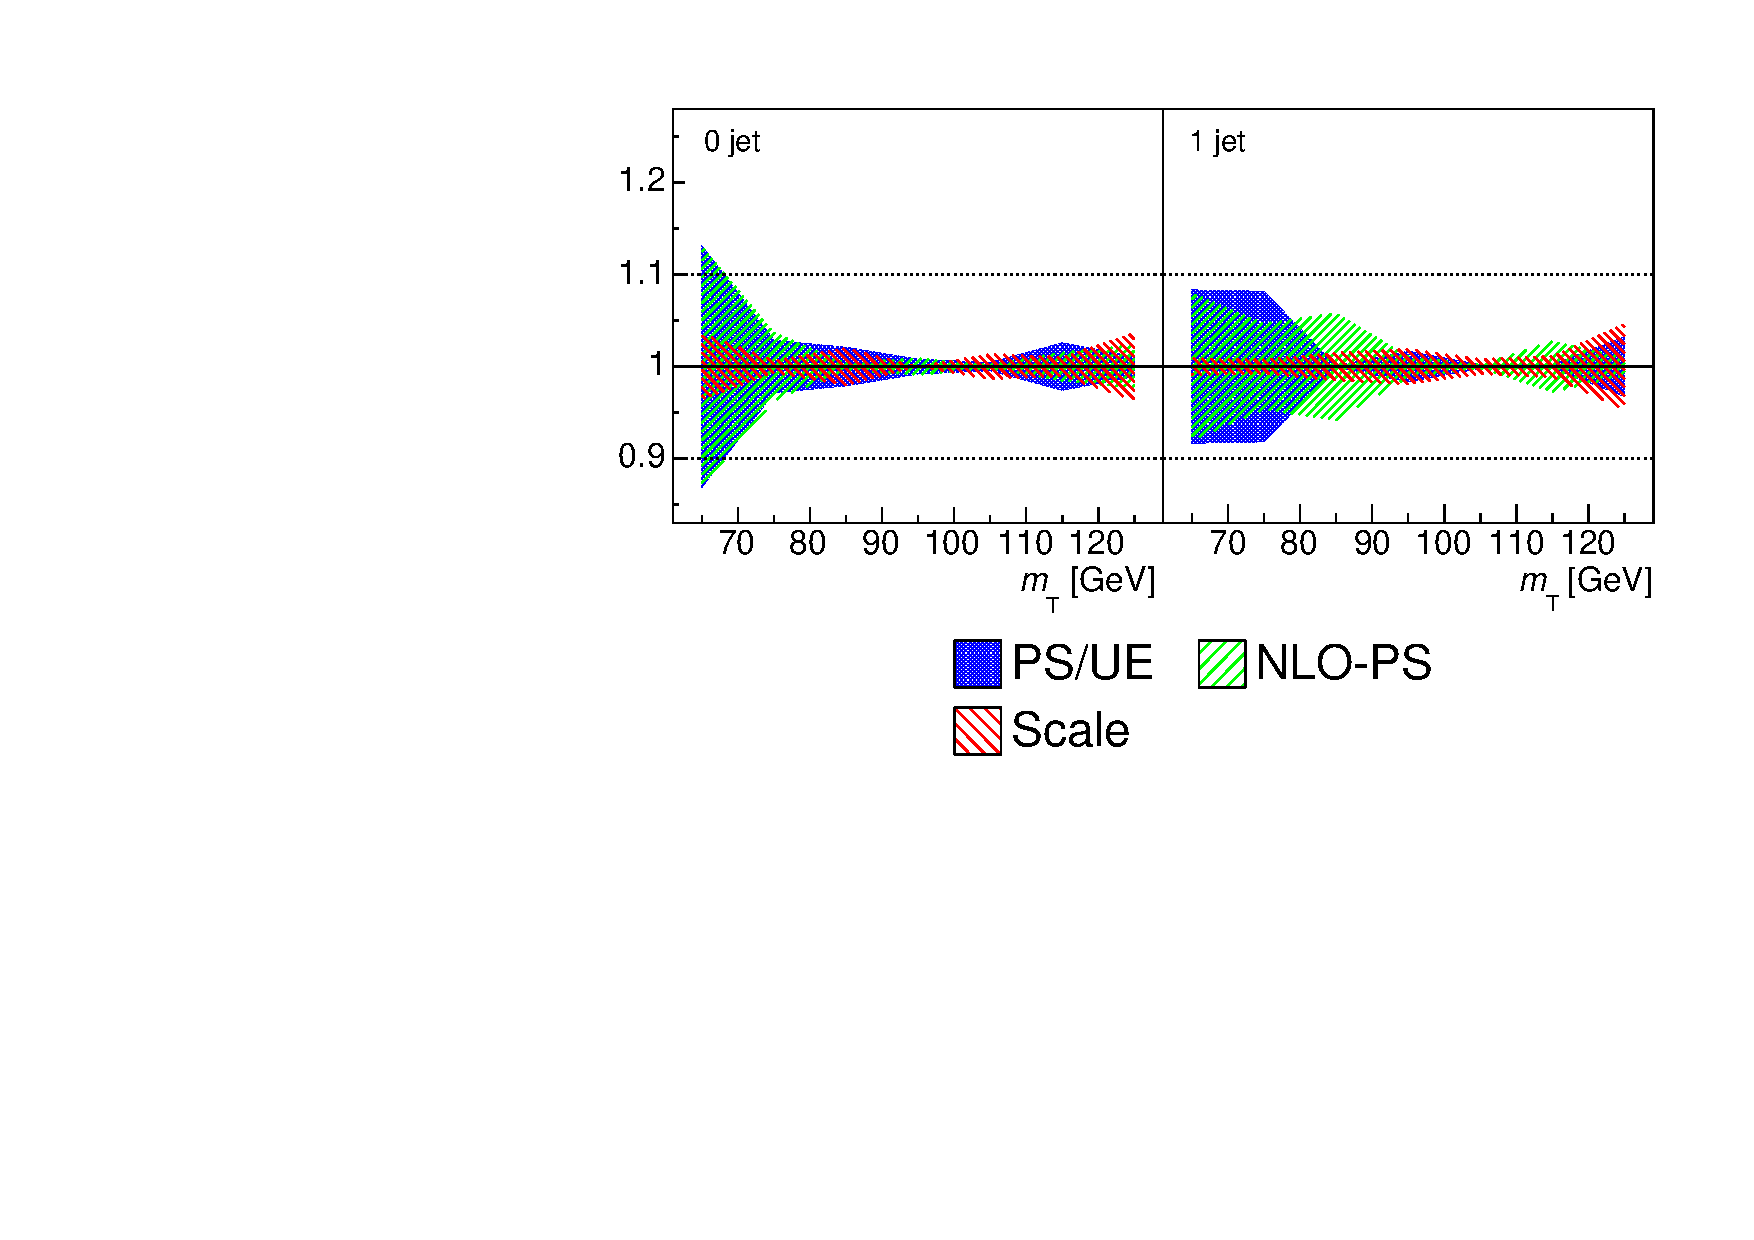
\includegraphics[width=\largefigwidth]{custom_images/mT-shapes/ggf}
	\\
	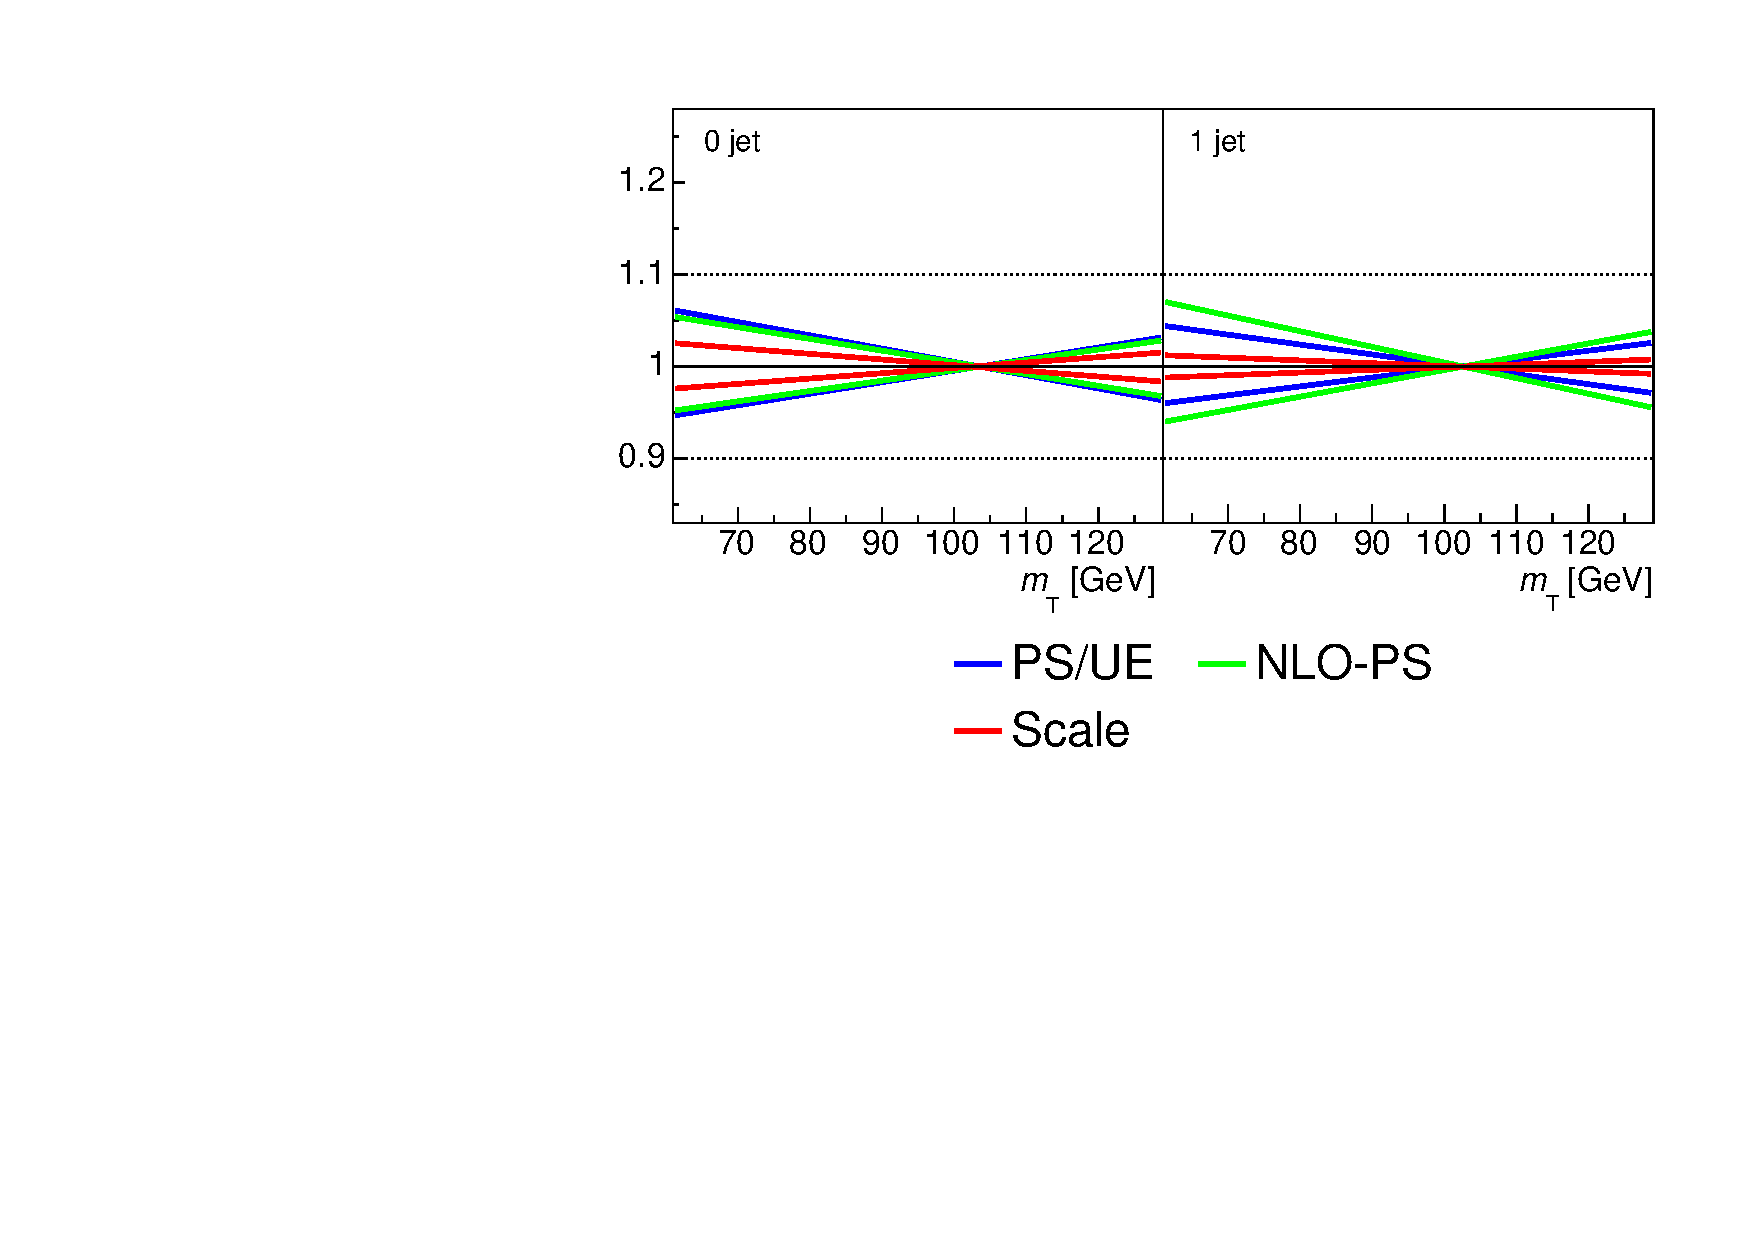
\includegraphics[width=\largefigwidth]{custom_images/mT-shapes/ggf_fits}
	\caption{ggF \mt shape systematic uncertainties in the 0-jet and 1-jet signal regions 
	of the \emch/\mech channels. The raw uncertainties are shown above and the fits are 
	shown below. The constant (flat) terms of the fit are outside the visible $x$-range.}
	\label{fig:signal:mTshape}
\end{figure}

